


%%%%%%%%%%%%%%%%%

\begin{frame}{A Path Forward}
 
 \begin{block}{Manage Complexity}
  \begin{itemize}
   \item Good interface design
   \item Refactor code when needed
   \item Hand-optimize small kernels only (cf.~BLIS methodology)
  \end{itemize}
 \end{block}
 
 \vspace*{-3.2cm}
 \begin{flushright}
  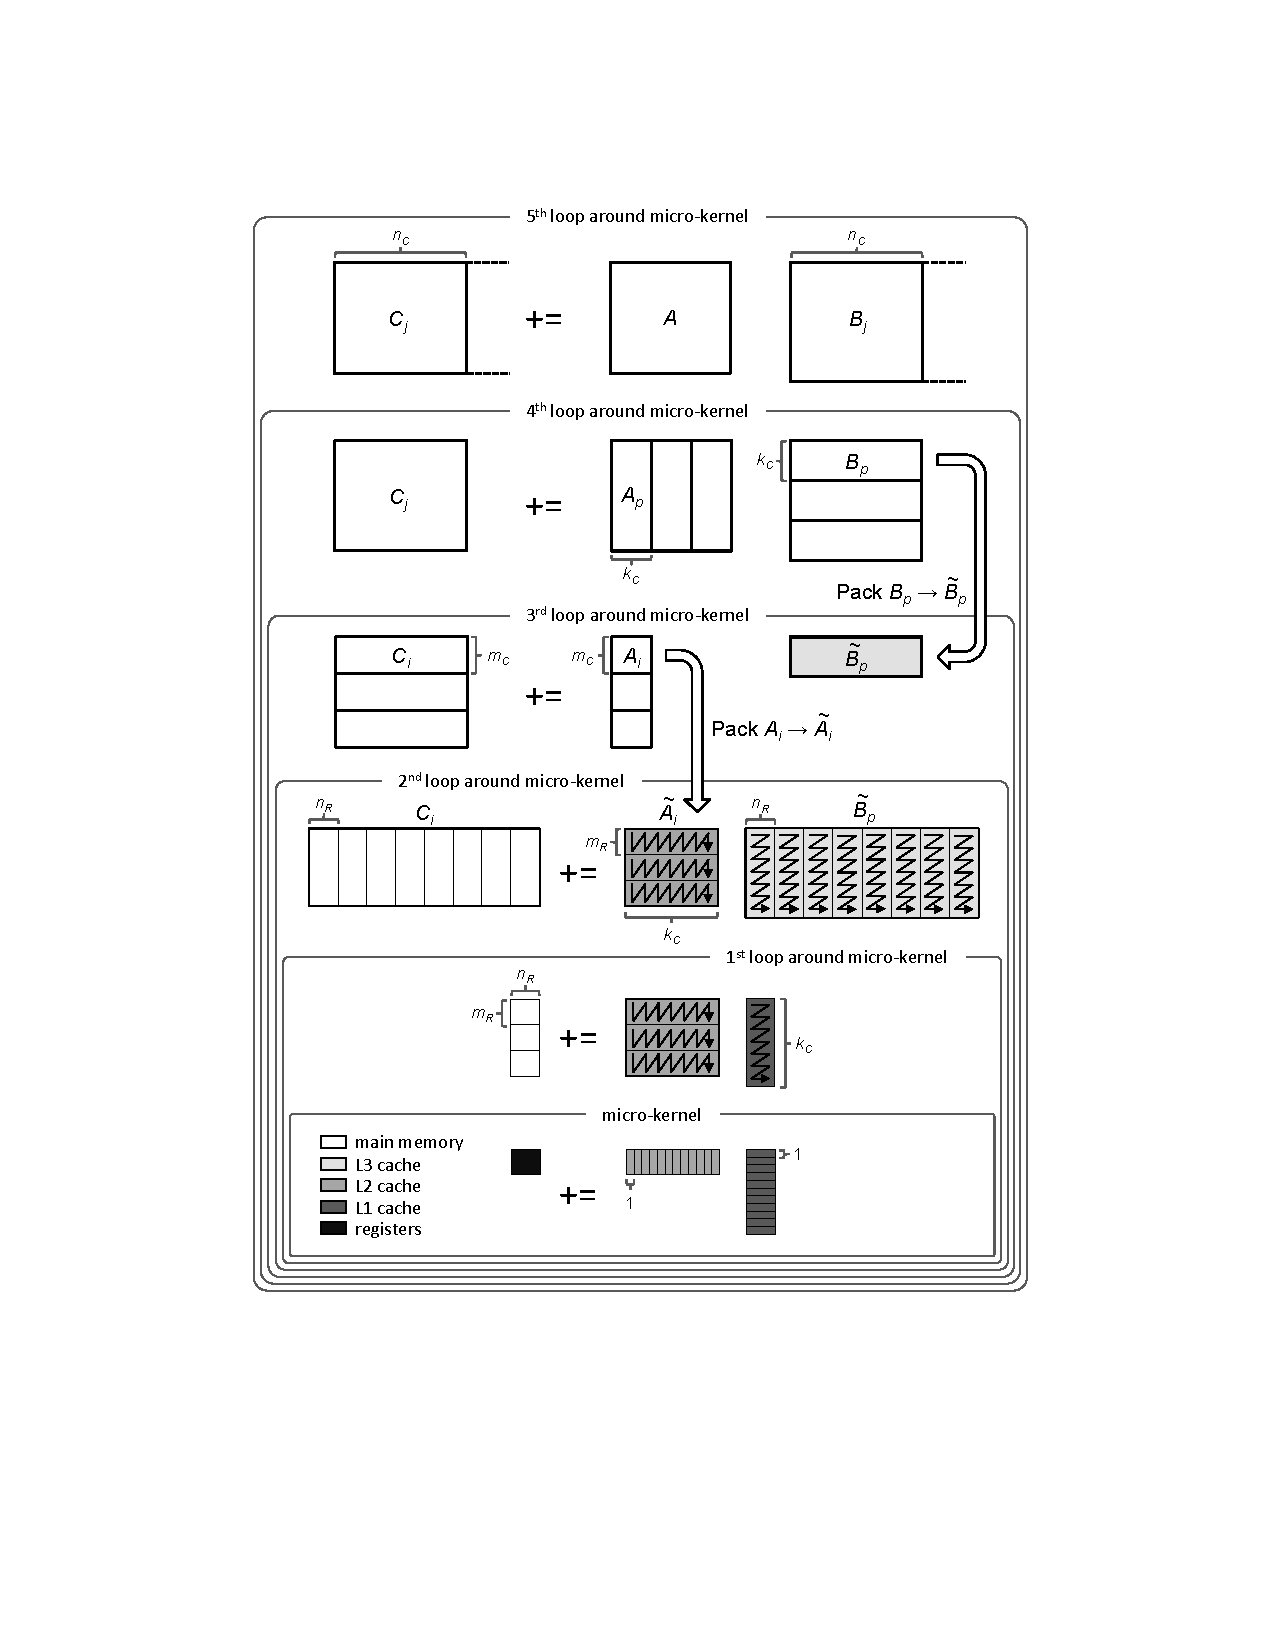
\includegraphics[width=0.36\textwidth]{figures/BLISLoops} \\
  {\scriptsize [F.~Van Zee, T.~Smith, ACM TOMS 2017]}
 \end{flushright}

 \vspace*{-4.5cm}
 %\pause
 \begin{block}{Development Implications}
  \begin{itemize}
   \item Adopt professional software development practices %(coding standards, rigorous testing, etc.)
   \item Develop, maintain, and evolve different datastructures ...
   \item ... and code paths
   \item Use clear and easy-to-understand datastructures
   \item Fallacy: ``Writing'' an application only once in its final form %and reusing it for decades is a fallacy
  \end{itemize}
 \end{block}
 
\end{frame}



%%%%%%%%%%%%%%%%%

\begin{frame}{A Path Forward}
 
 \begin{block}{Spending Development Resources}
  \begin{itemize}
   \item Reuse existing libraries --- reinventing the wheel is not productive!
   \item Focus on domain- and application-specific aspects
   \item Obtain expertise and resources for continuous code evolution
  \end{itemize}
 \end{block}

 %\pause
 \begin{block}{Required Incentives}
  \begin{itemize}
   \item Reward contributions to existing projects
   \item Pair research funding with software development funding
   \item Establish software development career tracks
  \end{itemize}
 \end{block}
 
\end{frame}


%%%%%%%%%%%%%%%%%

\begin{frame}{A Path Forward}
 
 \begin{block}{Is Performance Portability Just a Software Productivity Aspect?}
  \begin{center}
  \fbox{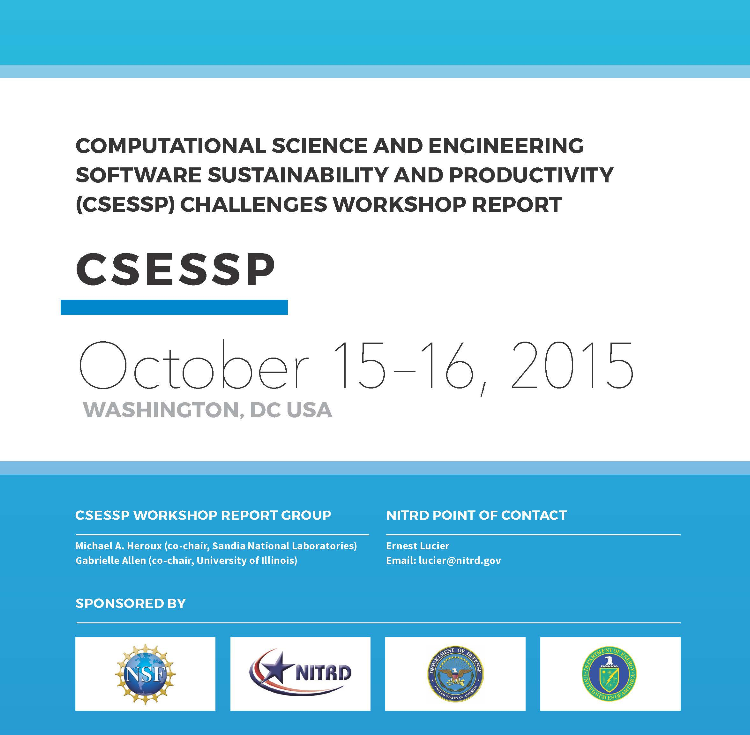
\includegraphics[width=0.4\textwidth]{figures/CSESSPWorkshopReport-front-page.png}} \\
  {\footnotesize \texttt{https://www.nitrd.gov/PUBS/CSESSPWorkshopReport.pdf}}
  \end{center}
 \end{block}
 
\end{frame}

